\documentclass[11pt,a4paper]{article}
\usepackage[top=3cm, bottom=2cm, left=2cm, right=2cm]{geometry}
\usepackage[utf8]{inputenc}
\usepackage{amsmath, amsfonts, amssymb}
\usepackage{siunitx}
\usepackage[brazil]{babel}
\usepackage{graphicx}
\usepackage[margin=10pt,font={small, it},labelfont=bf, textfont=it]{caption}
\usepackage[dvipsnames, svgnames]{xcolor}
\DeclareCaptionFont{MediumOrchid}{\color[svgnames]{MediumOrchid}}
\usepackage[pdftex]{hyperref}
\usepackage{natbib}
\bibliographystyle{plainnat}
\bibpunct{\textcolor{MediumOrchid}{\textbf{[}}}{\textcolor{MediumOrchid}{\textbf{]}}}{,}{s}{}{}
\usepackage{color}
\usepackage{footnote}
\usepackage{setspace}
\usepackage{booktabs}
\usepackage{multirow}
\usepackage{subfigure}
\usepackage{fancyhdr}
\usepackage{leading}
\usepackage{indentfirst}
\usepackage{wrapfig}
\usepackage{mdframed}
\usepackage{etoolbox}
\usepackage[version=4]{mhchem}
\usepackage{enumitem}
\usepackage{caption}
\usepackage{titlesec}
\usepackage{tcolorbox}
\usepackage{tikz}
\usepackage{LobsterTwo}
\usepackage[T1]{fontenc}
\usepackage{fontspec}
\usepackage{txfonts}
\usepackage[bottom]{footmisc}
\tcbuselibrary{skins,breakable}
\sisetup{output-decimal-marker={.}}

\makeatletter
\def\footnoterule{\kern-3pt\color{MediumOrchid}\hrule\@width0.6\textwidth height 0.8pt\kern2.6pt}
\makeatother

\renewcommand{\footnotelayout}{\itshape\color{MediumOrchid}}

\AtBeginEnvironment{equation}{\fontsize{13}{16}\selectfont}


\titleformat{\section}{\LobsterTwo\LARGE\color{CarnationPink}}{\thesection.}{1em}{}
\titleformat{\subsection}{\LobsterTwo\LARGE\color{CarnationPink}}{\thesubsection}{1em}{}
\titleformat{\subsubsection}{\LobsterTwo\large\color{MediumOrchid}}{\thesubsubsection}{1em}{}


\DeclareCaptionLabelFormat{figuras}{\textcolor{DarkTurquoise}{Figura \arabic{figure}}}
\captionsetup[figure]{labelformat=figuras}

\makeatletter
\renewcommand\tagform@[1]{\maketag@@@{\color{CarnationPink}(#1)}}
\makeatother

\renewcommand{\theequation}{Eq. \arabic{equation}}
\renewcommand{\thefigure}{Fig. \arabic{figure}}
\renewcommand{\thesection}{\textcolor{CarnationPink}{\arabic{section}}}

\setlist[itemize]{label=\textcolor{CarnationPink}{$\blacksquare$}}

\setlist[enumerate]{label=\textcolor{CarnationPink}{\arabic*.}, align=left, leftmargin=1.5cm}


\newcounter{exemplo}

\NewDocumentEnvironment{exemplo}{ O{} }{%
\allowbreak
\setlength{\parindent}{0pt}
  \begin{mdframed}[
  leftline=true,
  topline=false,
  rightline=false,
  bottomline=false,
  linewidth=2pt,
  linecolor=CarnationPink,
  frametitlerule=false,
  frametitlefont=\LobsterTwo\large\color{CarnationPink},
  frametitle={\color{CarnationPink}\LobsterTwo\large #1},
  ]
}{%
  \end{mdframed}
}

\setlength{\fboxsep}{5pt}
\setlength{\fboxrule}{1.5pt}
\usepackage{float}
\renewcommand{\thefootnote}{\alph{footnote}}
\usepackage{url}
\hypersetup{
	colorlinks=true,
	linkcolor=DarkTurquoise,
	filecolor=DarkTurquoise,      
	urlcolor=DarkTurquoise,
	citecolor=DarkTurquoise,
	pdftitle={Especialista em Física da Radioterapia}
}
\pagestyle{fancy}
\fancyhf{}
\renewcommand{\headrulewidth}{0pt}
\rfoot{Página \thepage}

\title{\LobsterTwo\Huge{Braquiterapia}}
\author{\LobsterTwo\Large{Braquiterapia Oftalmológica e Intravascular\nocite{*}}}
\date{\LobsterTwo\textit{Dalila Mendonça}}
\begin{document}
	\maketitle

\section{Braquiterapia Ocular}

\subsection*{Tumores Oculares}

    Tumores oculares, predominantemente melanomas oculares e retinoblastomas, são tumores do olho que surgem na camada uveal\footnote{A camada uveal, também conhecida como trato uveal, é uma das estruturas do olho humano e está localizada entre a esclera (a parte branca do olho) e a retina (a camada sensível à luz). É composta por três partes principais: a íris, o corpo ciliar e a coroide.}. Tumores maiores são tratados com enucleação cirúrgica do olho, mas tumores menores geralmente são primeiramente irradiados afim de se preservar o olho e o máximo possível de visão funcional. Devido ao pequeno tamanho dos tumores oculares e a sua proximidade, praticamente imediata, com estruturas críticas do aparato óptico, os tratamentos devem atingir alta conformidade de dose e gradientes de dose acentuados, tipicamente associados à radiocirurgia estereotáxica (SRS) ou à braquiterapia. Em 2003, a American Brachytherapy Society (ABS) publicou recomendações clínicas para o tratamento de melanomas uveais.
    
    Em oftalmologia, a ultrassonografia fotográfica digital é normalmente usada para identificar a posição dos tumores oculares e medir sua dimensão. Isso pode ser complementado por um estudo de ressonância magnética (MRI) ou por tomografia computadorizada (TC).

\subsection*{Braquiterapia Oftalmológica}


    A braquiterapia oftamológica é utilizada para o tratamento de Melanomas Oculares ou melanomas coroidais e de retinoblastomas (mais comum em pacientes neonatais e bebês). Os primeiros tratamentos de braquiterapia oftalmológica eram realizados com Cobalto-60 e subsequentemente foram testadas outras fontes como o Irídio-192, Rutênio-106, Iodo-125  Paládio-103, Estrôncio-90 e Césio-131.  Antes de 2002 os guidelines eram focados no Iodo-125 mas conforme outras fontes foram sendo utilizadas, novos protocolos foram estabelecidos pela American Brachyterapy Society. 
    
    A braquiterapia na forma de placas oculares tem sido uma opção de tratamento bem-sucedida e amplamente utilizada no tratamento de melanomas oculares. Essa abordagem terapêutica baseia-se em um estudo clínico chamado Collaborative Ocular Melanoma Study (COMS), que foi um estudo multicêntrico e randomizado.

    O COMS foi um estudo clínico de grande escala que teve como objetivo comparar a eficácia da enucleação (remoção cirúrgica do olho) com a irradiação (braquiterapia com placas oculares) no tratamento de melanomas oculares. O estudo envolveu a participação de vários centros de pesquisa e foi conduzido ao longo de muitos anos. Uma das principais contribuições do COMS foi o desenvolvimento e a padronização das placas de braquiterapia para o tratamento de melanomas oculares (\ref{fig:coms}). Essas placas são dispositivos projetados para se encaixarem na superfície externa do olho, fornecendo uma distribuição precisa de radiação para o tumor ocular. As placas contêm pequenas fontes radioativas, como o Iodo-125, que emitem radiação de baixa energia para o tratamento do melanoma ocular.

    \begin{figure}[h]
        \centering
        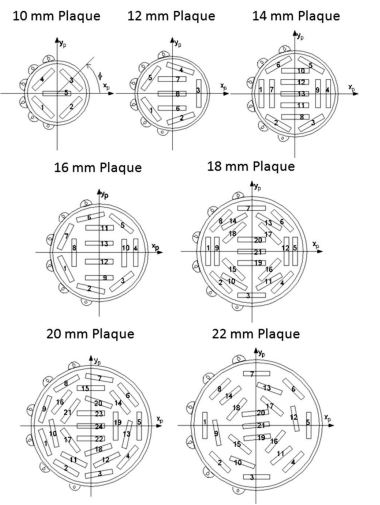
\includegraphics[width=0.6\textwidth]{Imagens/placasComs.JPG}
        \caption{Diagrama das sementes distribuídas em placas COMS. Consistem em um suporte feito de uma liga de ouro com um portador de sementes feitos de Silastic(borracha de silicone) acoplados no suporte.}
        \label{fig:coms}
    \end{figure}

    O estudo COMS demonstrou que a irradiação com placas oculares é uma alternativa eficaz à enucleação para o tratamento de melanomas oculares de tamanho médio a grande. Os resultados mostraram taxas semelhantes de controle local do tumor e sobrevida global entre os dois grupos de tratamento. Além disso, a irradiação com placas oculares preservou o olho e a visão funcional em muitos casos, oferecendo aos pacientes uma melhor qualidade de vida.

    Desde o estudo COMS, as placas de braquiterapia se tornaram uma opção padrão de tratamento para melanomas oculares. A técnica de implantação das placas e o planejamento do tratamento são realizados por uma equipe multidisciplinar, incluindo oftalmologistas, radioterapeutas e físicos médicos. A escolha da placa adequada, o posicionamento preciso das fontes radioativas e a determinação da dose correta são fundamentais para garantir uma distribuição de dose adequada e um tratamento eficaz.
    
    Uma alternativa de tratamento é a radioterapia com feixes de prótons. Os feixes de prótons com energia de até 80 MeV são ideais para irradiação de melanomas oculares devido às suas características de deposição de dose e aos aspectos muito menos invasivos do procedimento comparado à braquiterapia oftalmológica. Os ensaios clínicos indicam que os feixes de prótons são mais úteis para tumores grandes e/ou localizados mais posteriormente, mas o uso de feixes de prótons tem sido historicamente muito limitado devido à pouquíssima disponibilidade de feixes clínicos de prótons. Com a recente proliferação de instalações clínicas de prótons, um número crescente de pacientes provavelmente será tratado usando essa modalidade. Da mesma forma, a acessibilidade mais ampla a máquinas de tratamento SRS dedicadas levou ao desenvolvimento de tratamentos SRS de fração única utilizando o Gamma Knife ou CyberKnife. A imobilização do tumor para tratamentos com prótons ou SRS pode ser obtida por meio de dois métodos:

    \begin{enumerate}
        \item Exigir que o paciente olhe para um ponto fixo definido na sala de tratamento. Isso requer a cooperação do paciente; o posicionamento do olho pode ser verificado usando um sistema de raios-x para identificar marcadores fiduciais costurados na órbita.
        \item Paralisar a musculatura ocular injetando anestesia local. A medicação age como um bolus e muda ligeiramente a posição do olho; a imagem de simulação, o planejamento do tratamento e a administração do tratamento devem ser realizados antes que o agente anestésico seja reabsorvido no corpo, geralmente dentro de 2 a 3 horas.
    \end{enumerate}
    

\subsection*{Critério de Exclusão para Braquiterapia Com Placas Oftálmicas}

    Existem alguns critérios de exclusão para o uso da braquiterapia com placas oftálmicas no tratamento de melanomas oculares. Esses critérios são baseados nas características do tumor e nas limitações da técnica de braquiterapia. Alguns desses critérios são:

    \begin{itemize}
        \item Extensão extraocular grosseira (T4e) ou tamanho do tumor: A braquiterapia com placas oftálmicas é mais adequada para tumores de tamanho médio a grande, geralmente até \SI{5}{\centi\meter} de diâmetro basal. Tumores com extensão extraocular significativa, ou seja, que se estendem para fora do globo ocular de forma extensa, podem não ser adequados para o tratamento com placas oftálmicas. Nesses casos, outras abordagens terapêuticas, como a enucleação, podem ser consideradas.
        
        \item Diâmetros basais que excedem os limites de braquiterapia: As placas oftálmicas têm tamanhos e formatos específicos que limitam o diâmetro basal do tumor que pode ser tratado efetivamente. Se o tumor exceder os limites estabelecidos pelas placas disponíveis, outras opções de tratamento podem ser consideradas.
        
        \item Olho doloroso cego e sem percepção de luz: Em alguns casos, quando o olho afetado pelo melanoma está associado a dor persistente e perda total da visão (sem percepção de luz), o tratamento com placas oftálmicas pode não ser adequado. Nesses casos, outras opções de tratamento, como a enucleação, podem ser recomendadas para aliviar a dor e melhorar a qualidade de vida do paciente.
        \end{itemize}

\subsection*{Possíveis reações}


    \begin{itemize}
        \item Efeitos tardios - predominantes: Retinopatia radio-induzida, catarata, necrose escleral, Vazamento vascular periférico da retina com exsudação e hemorragia.
        \item Tumores próximos a fóvea ocular e ao nervo ótico podem causar morbidades como a cegueira. Quanto maior a distância entre a placa e a mácula ou o nervo ótico melhor o resultado visual.
        \item É possível evitar a incidência de retinopatia por radiação e neuropatia ótica aplicando injeções intravítreas de triancinolona e agentes anti-fator de crescimento endotelial vascular
    \end{itemize}

\subsection*{Tratamento}

    O tratamento de braquiterapia com placas oculares é uma abordagem eficaz para o tratamento de tumores intraoculares, como melanomas oculares. O documento colaborativo entre a American Brachytherapy Society (ABS) e a American Association of Physicists in Medicine (AAPM) chamado TG-129 aborda a dosimetria das placas oftálmicas COMS, que são utilizadas com as fontes radioativas de \ce{^{125}I} e \ce{^{103}Pd}.

    A prescrição típica de dose para o tratamento com placas oculares é de 85 Gy em um ponto a 5 mm de profundidade. Essa dose é projetada para fornecer um nível efetivo de tratamento para o tumor intraocular, enquanto minimiza a dose nos tecidos saudáveis circundantes. O diâmetro da placa ocular a ser utilizada é determinado pelo diâmetro máximo do tumor, garantindo uma cobertura adequada da região afetada.

    As placas oculares consistem em um molde de metal redondo ou oval, com diâmetro variando de 8 mm a 20 mm. Essas placas são feitas de materiais biocompatíveis e possuem um suporte de liga de ouro, que fornece proteção ao tecido normal adjacente durante o tratamento. Elas possuem inserções de silicone (Silastic) padrão ou personalizáveis para a colocação das sementes radioativas.

    As sementes radioativas, contendo as fontes de \ce{^{125}I}, \ce{^{103}Pd} ou, menos comumente, \ce{^{131}Cs}, são fixadas nos slots projetados especificamente na placa ocular. Em seguida, as sementes são cobertas com o suporte de ouro, proporcionando uma distribuição de dose adequada ao tumor. Antes do procedimento, as placas oculares e as sementes são esterilizadas para garantir a segurança e a eficácia do tratamento.

    No caso de tumores próximos ou adjacentes ao nervo óptico, é utilizada uma placa "entalhada", projetada com um entalhe que se encaixa ao redor do nervo óptico, garantindo a proteção adequada desse tecido crítico.

    Após a fixação da placa ocular, o paciente permanece internado por um período de 3 a 7 dias, durante os quais o tratamento é administrado. Após esse período, a placa ocular é removida cirurgicamente. A escolha entre \ce{^{125}I} e \ce{^{103}Pd} como fontes de baixa taxa de dose depende de vários fatores, como o tamanho e a localização do tumor, a geometria do olho e a experiência da equipe médica. Ambas as fontes têm sido amplamente utilizadas e mostraram eficácia no tratamento de melanomas oculares.O tratamento de braquiterapia com placas oculares é uma abordagem eficaz para o tratamento de tumores intraoculares, como melanomas oculares. O documento colaborativo entre a American Brachytherapy Society (ABS) e a American Association of Physicists in Medicine (AAPM) chamado TG-129 aborda a dosimetria das placas oftálmicas COMS, que são utilizadas com as fontes radioativas de \ce{^{125}I} e \ce{^{103}Pd}.

    Durante o processo de planejamento do tratamento de braquiterapia com placas oculares, diversos parâmetros são considerados para garantir uma cobertura adequada do tumor. A localização das sementes radioativas, a intensidade dessas sementes e a duração do tratamento são determinadas com base nas características do tumor e nas metas de dose estabelecidas.

    A profundidade do tumor é um parâmetro crucial, pois influencia diretamente a distribuição de dose. O protocolo COMS estabelece uma profundidade de 5 mm como referência, mas em casos de tumores maiores, essa profundidade pode ser modificada para garantir uma dose adequada ao tumor. Além disso, a margem basal, que é a extensão do tumor em sua base, também é um fator importante a ser considerado. Embora o protocolo COMS especifique uma margem basal de 3 mm, estudos mais recentes indicam que uma margem de 5 mm é necessária para garantir uma cobertura tumoral suficiente.

    Os cálculos de dose na braquiterapia oftálmica são altamente sensíveis a vários fatores, como o modelo da semente, o desenho da placa e a presença de heterogeneidades no meio. Devido à baixa energia dos fótons emitidos pelas fontes utilizadas, os algoritmos de cálculo de dose, como o TG-43 da AAPM (American Association of Physicists in Medicine), podem apresentar diferenças significativas quando comparados a métodos mais avançados, como a modelagem de Monte Carlo ou técnicas de rastreamento de raios, que levam em consideração a heterogeneidade dos tecidos.

    Estudos comparativos mostraram que os cálculos de dose usando o algoritmo TG-43 para fontes pontuais e fontes lineares em meios homogêneos concordam dentro de alguns pontos percentuais com a dose no eixo central. No entanto, quando a heterogeneidade dos tecidos é considerada nos cálculos, por meio de modelagem de Monte Carlo ou técnicas de rastreamento de raios, podem ser observadas diferenças significativas de 37\% ou mais entre os métodos. Essas diferenças ressaltam a importância de utilizar métodos mais avançados de cálculo de dose, especialmente quando há presença de heterogeneidades no olho ou nos tecidos circundantes. Previamente aos rápidos desenvolvimentos de métodos aprimorados para cálculo de dose em braquiterapia, o AAPM TG-129, \textbf{``Dosimetry of 125I and 103Pd COMS Eye Plaques for Intraocular Tumores''}, recomenda:

    \textit{\textbf{\textcolor{MediumOrchid}{Antecipando ao TPS de braquiterapia que permite cálculos de dose heterogênea, por exemplo, correção semi-analítica do comprimento do caminho, MC, cone colapsado, ordenadas discretas ou outras abordagens, a AAPM e a ABS recomendam a realização de um cálculo ou estimativa de dose paralelo para incluir os efeitos de heterogeneidades do material da placa quando esses TPS de braquiterapia estiverem disponíveis. No mínimo, deve-se obter a dose corrigida pela heterogeneidade para o ponto de prescrição, mas preferencialmente uma distribuição de dose 2D.}}}

    Para o comissionamento de um programa de braquiterapia baseados em placas oftalmológicas utilizando um sistema de planejamento de tratamento 3D, os guidelines existentes para os sistemas guiados por imagem utilizados no planejamento de tratamento baseados em ultrassom, TC ou RM devem ser seguidos. A calibração e o ensaio de sementes de braquiterapia de baixa taxa de dose são descritos no report da AAPM \textbf{``Low Energy Brachytherapy Source Calibration Working Group''}.

\subsection*{Planejamento de Tratamento} 


\begin{itemize}
    \item É necessário obter informações do oftalmologista, como a lateralidade do tumor (se é no olho direito ou esquerdo), o estágio do tumor e o tamanho (diâmetro e altura). Essas informações são confirmadas por meio de exames de ultrassom e um diagrama de fundo detalhado, que mostra a localização do tumor, as medidas tumorais e a distância do tumor em relação a várias estruturas oculares importantes, como a fóvea, nervo óptico, glândula lacrimal, cristalino e o olho oposto.
    
    \item Os dados do diagrama de fundo são transferidos para o sistema de planejamento de tratamento (TPS), onde são inseridos os dados dosimétricos da fonte de radiação escolhida para o procedimento. Com base nesses dados, a dose no tumor e a dose nos órgãos em risco (OAR) são calculadas, levando em consideração as diretrizes estabelecidas pelo estudo COMS (Collaborative Ocular Melanoma Study) e pelo TG-129.
    
    \item Os diâmetros do tumor devem ser menores que o alvo de tratamento (PTV) ou o diâmetro da placa oftálmica para evitar perdas geográficas. Isso garante que a dose seja entregue adequadamente ao tumor, evitando a exposição desnecessária de tecidos normais circundantes.
    
    \item O ponto de prescrição da dose deve ser no ápice do tumor, que é o ponto de espessura máxima. Isso garante que a dose seja entregue diretamente na região de interesse, onde o tumor está localizado.
    
    \item É importante que a isodose de prescrição cubra todo o tumor para maximizar o controle local. A isodose de prescrição é a linha que delimita a região onde a dose prescrita é alcançada. Garantir a cobertura completa do tumor ajuda a maximizar a eficácia do tratamento.
    
    \item Para o tratamento de retinoblastoma, a prescrição de dose geralmente varia de 40 Gy a 45 Gy, a serem entregues ao longo de 1 a 5 dias.
    
    \item A dose total no ápice tumoral pode variar, dependendo do radionuclídeo escolhido, mas geralmente varia de 70 Gy a 100 Gy nos casos de melanoma. Essa alta dose é necessária para garantir a destruição eficaz das células tumorais.
    
    \item A prescrição de dose comum para melanoma coroidial é de 85 Gy em uma profundidade mínima de 5 mm. Isso é realizado utilizando uma placa oftálmica com uma margem de 0.3 cm em torno do diâmetro basal do tumor. Essa dose é entregue em um período de 3 a 7 dias consecutivos.
    
    \item Existe um gradiente de dose que varia com a profundidade do tratamento e dependendo do radionuclídeo utilizado. Isso significa que a dose máxima pode variar em diferentes profundidades do tumor.
    
    \item A prescrição de dose mencionada para melanoma coroidial é baseada em um meio homogêneo. Em um meio homogêneo, a prescrição de 85 Gy a 10 mm de profundidade resultará em uma dose máxima (Dmax) de 644 Gy no interior da esclera, a 3 mm de profundidade a Dmax será de 166 Gy e a 5 mm de profundidade a Dmax será de 260 Gy.
    
    \item Emissores beta, como Ru-106 e Rh-106, são indicados para tratar lesões com espessura do ápice menor que 5-6 mm. Eles possuem uma característica única de emissão de partículas beta, que têm um alcance curto no tecido, permitindo uma alta dose concentrada na região do tumor.
    
    \item As placas de 106-Ru são finas, com cerca de 1 mm de espessura. Isso permite uma colocação precisa e um perfil de dose adequado para o tratamento de melanomas oculares.
    
    \item Fontes de radiação como \ce{^{103}Pd} (com energia de 21 keV), \ce{^{125}I} (com energia de 28 keV) e \ce{^{131}Cs} (com energia de 30 keV) apresentam um aumento progressivo do gradiente de dose do menor para o maior. Isso significa que a dose aumenta na esclera (tecido circundante) e diminui nas estruturas oculares normais.
    
    \item O uso de métodos de cálculo heterogêneos, que levam em consideração as heterogeneidades dos tecidos, pode resultar em uma diferença de dose superior a 10\% em comparação com os cálculos em meios homogêneos. É importante considerar as heterogeneidades no planejamento do tratamento para garantir uma dose precisa no tumor e uma preservação adequada dos tecidos normais.
    
    \item A taxa de dose não deve ser menor que o padrão COMS equivalente de 0.60 Gy/h para o \ce{^{125}I}. Essa taxa de dose é importante para garantir que a dose seja entregue de forma eficaz ao longo do tempo necessário para o tratamento.
    
    \item A atividade típica de \ce{^{125}I} usada por semente varia entre 0.5 e 5 mCi para alcançar taxas de dose entre 0.5 e 1.25 Gy/h. A seleção da atividade adequada depende do objetivo de dose desejado e do tempo total de tratamento.
    
    \item A localização do tumor pode ser feita utilizando técnicas como fundoscopia, fotografia de fundo e ultrassom. Essas técnicas ajudam a identificar a posição exata do tumor no olho. Além disso, tomografia computadorizada (CT) e ressonância magnética (RM) também podem ser utilizadas para auxiliar na localização da lesão. Após o implante das placas oftálmicas, a verificação da posição das placas é feita com o uso de ultrassom.
    
    \item Além das fontes já mencionadas, outras fontes radioativas, como \ce{^{90}Sr} e \ce{^{90}Y} (emissores beta) e \ce{^{60}Co}, também podem ser utilizadas em casos específicos, dependendo das necessidades e características do tumor.
    \end{itemize}


\subsection*{Cirurgia}

    Durante o procedimento cirúrgico para a braquiterapia ocular, é recomendado que uma equipe multidisciplinar, composta por oncologista oftalmológico, radio-oncologista e físico médico, trabalhe em conjunto. Cada membro da equipe desempenha um papel importante na garantia de um tratamento eficaz e seguro.

    \begin{wrapfigure}{r}{0.48\textwidth}
        \centering
        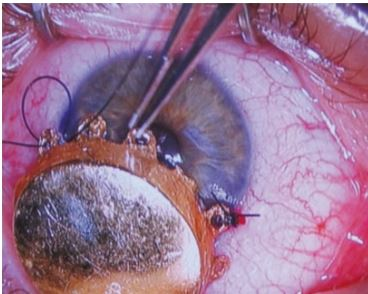
\includegraphics[width=0.45\textwidth]{Imagens/placaComsOuroMC.JPG}
        \caption{Fotografia externa da placa COMS feita de uma liga de ouro, costurada na esclera após a localização.}
    \end{wrapfigure}

    O cirurgião oftalmológico localiza o tumor e faz as medições necessárias para determinar o diâmetro da placa ocular que será utilizada. Essa seleção leva em consideração o tamanho do tumor e a margem de planejamento necessária para garantir a cobertura adequada do tumor durante o tratamento.

    Após a seleção da placa ocular adequada, ela é fixada na esclera, que é o tecido fibroso que reveste o olho. Isso é feito por meio de suturas cuidadosamente colocadas. Em alguns casos, pode ser necessário realocar um músculo ocular para permitir a inserção correta da placa. Essa realocação é realizada para garantir que a placa fique adequadamente posicionada e em contato com o tumor.

    Durante o procedimento cirúrgico, o tempo de inserção da placa é registrado no relatório médico para fins de documentação e controle de qualidade. Após a colocação da placa, um tapa olho de chumbo é colocado sobre o olho afetado para proteger o paciente da radiação durante o período de tratamento.

    A placa ocular permanece no local durante todo o período pré-planejado, fornecendo a dose apropriada de radiação na profundidade necessária para tratar o tumor. Essa duração varia de acordo com o protocolo específico estabelecido para cada caso.

    Ao final do tratamento, a placa ocular é removida sob anestesia local. Se algum músculo ocular foi realocado durante a inserção da placa, ele é colocado novamente em sua posição original. Todo o processo cirúrgico é realizado com cuidado para garantir a precisão e a segurança do tratamento.

   
    \begin{figure}[h]
        \centering
        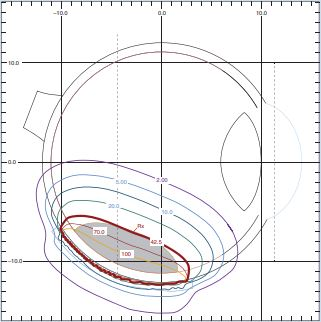
\includegraphics[width=0.35\textwidth]{Imagens/distribDosePlacaOftamRutenio.JPG}
        \caption{Distribuição de Isodose para uma Placa de Rutênio de 15.3mm modelo CCA, onde o alvo é a sombra cinza. Devido ao acentuado falloff de dose a profundidade de tratamento dessas placas são limitadas entre 5-6 mm a partir da superfície da placa.}
    \end{figure}
 

    \begin{figure}[h]
        \centering
        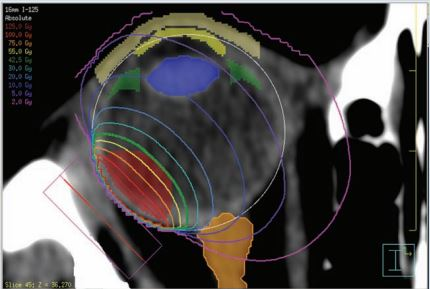
\includegraphics[width=0.4\textwidth]{Imagens/distribDosePlacaComsI125.JPG}
        \caption{Corte axial de TC mostrando a distribuição de isodose para uma placa de Iodo-125 COMS de 16 mm para entregar 42.5Gy no alvo (em vermelho). O perfil de dose baseado em Monte-Carlo, que considera os efeitos da capa de ouro e a atenuação nos portadores de silicone, foi atribuído à fonte, representada pelo retângulo.}
    \end{figure}

% TODO: pegar dados no TG 129 e no guideline da ABS

\section{Microesferas}

    A braquiterapia com microesferas utilizando a emissão de partículas beta do \ce{^{90}Y} (ítrio) é utilizada no tratamento de malignidades hepáticas. O \ce{^{90}Y} é embalado em pequenas microesferas de vidro com 20 \unit{\mu m} a 60 \unit{\mu m} de diâmetro, que são injetadas na artéria hepática. A maioria dos tratamentos ocorre em departamentos de radiologia intervencionista com o apoio do físico especialista em medicina nuclear. Em clínicas menores, o fisioterapeuta pode precisar realizar esse procedimento; Como em todos os procedimentos especiais, recomenda-se a supervisão de um físico experiente e/ou obter treinamento do fornecedor dedicado à aplicação de microesferas. Como material de subproduto radioativo, o uso de microesferas de braquiterapia 90Y é regulamentado em 10 CFR 35 para estados de acordo nos Estados Unidos. A Nuclear Regulatory Commission (NRC) também fornece material de orientação adicional em seu site \href{http://www.nrc.gov/materials/miau/med-use-toolkit.html#other}{http://www.nrc.gov/materials/miau/med-use-toolkit}

    A braquiterapia com microesferas utiliza o duplo suprimento sanguíneo do fígado através da artéria hepática e da veia porta-hepática. Os tumores hepáticos metastáticos e os carcinomas hepatocelulares maiores que 3 mm de diâmetro recebem 80\% a 90\% de seu suprimento sanguíneo através da artéria hepática, enquanto a veia porta-hepática fornece $\approx$80\% para o tecido hepático normal. Portanto, as fontes emissoras de radiação administradas através da artéria hepática visarão principalmente as malignidades hepáticas, com doses relativamente pequenas sendo depositadas no tecido hepático normal. A fonte \ce{^{90}Y} é embalada em microesferas de vidro ou resina biocompatível de 20 \unit{\mu m} a 60 \unit{\mu m} de diâmetro em uma solução de água esterilizada. A administração das microesferas causa tanto uma embolização do suprimento sanguíneo do tumor quanto uma entrega de dose de radiação localizada, combinando danos isquêmicos e os danos devido à radiação no tumor.

    O AAPM TG-144 com respeito a dosimetria, imagem e controle de qualidade de braquiterapia com microesferas de \ce{^{90}Y} no tratamento de malignidades hepáticas fornece uma boa introdução sobre a justificativa, sobre as fontes comercialmente disponíveis, sobre os protocolos de imagem e os aspectos regulatórios. O guideline ACR-ASTRO-SIR com respeito a radioembolização com através de braquiterapia de microesferas (RMBD) para o tratamento de malignidades hepáticas abrange as qualificações da equipe, diretrizes de procedimento relacionadas à atividade das fontes e sua administração, bem como questões de segurança pessoal. Além disso, o Consórcio Oncológico de Braquiterapia por Radioembolização publicou um report contendendo recomendações que resumem o estado da arte atual do conhecimento sobre a segurança e a eficácia da braquiterapia com microesferas.

    Um grande desafio em todas os tratamentos hepáticos, incluindo a braquiterapia com microesferas, é com respeito a imagem do fígado. A complexidade do órgão e sua alta vascularização requerem protocolos de imagem bem desenvolvidos para garantir o diagnóstico preciso da carga tumoral. Na maioria dos casos, uma TC trifásica (isto é, uma TC sem contraste seguida por uma TC com contraste em dois intervalos de tempo definidos) é frequentemente complementada com uma tomografia por emissão de pósitrons (PET)/TC e, se disponível, um estudo de RM. Quando combinados, esses estudos fornecerão o volume do tumor necessário para o planejamento do tratamento. Uma angiografia pré-tratamento é necessária, além da imagem de simulação, para determinar o fluxo sanguíneo hepático e o trajeto do cateter para o procedimento. Ao mesmo tempo deste angiograma de pré-tratamento, uma embolização dos vasos extra-hepáticos é realizada para evitar depósitos de microesferas fora do fígado. Essa embolização é seguida por uma administração de \ce{^{99m}Tc}-MAA (albumina agregada), que pode ser visualizado usando uma gama câmera para prever a administração da dose das microesferas. A albumina agregada destina-se a substituir a biodistribuição da microesfera e os resultados de imagem de \ce{^{99m}Tc}-MAA determinam a quantidade de dose que foi desviada para os pulmões.

    A dosimetria da braquiterapia com microesferas é baseada na suposição de captação uniforme no fígado e no tecido tumoral, subtraído a dose que foi desviada para os pulmões, conforme determinado pela imagem de SPECT pré-tratamento. O padrão para a dosimetria de braquiterapia com microesferas foi desenvolvido pelo Comitê de Dose de Radiação Interna Médica (MIRD) da Sociedade de Medicina Nuclear. Esses modelos de cálculo de dose mais simples foram recentemente complementados pela disponibilidade da modelagem de dose 3D baseada em imagens utilizando dosimetria de convolução de kernel, com o kernel de dose determinado por simulação de Monte Carlo (MC). A imagem planar ou SPECT durante o procedimento pode fornecer confirmação da localização da administração da dose.

    Atualmente, não há um padrão rastreável pelo Instituto Nacional de Padrões e Tecnologia (NIST) para braquiterapia com microesferas de \ce{^{90}Y}. O ensaio da atividade das fontes de \ce{^{90}Y}, portanto, seguirá o respectivo protocolo do fornecedor e usará uma amostra da atividade de referência fornecida pelo fornecedor. As leituras da atividade em dosímetros utilizados na medicina nuclear são muito sensíveis à localização geométrica da fonte dentro do detector e à distribuição das microesferas dentro de seus respectivos portadores de fonte ativa. Portanto, é necessário seguir de perto as recomendações do fornecedor sobre as medidas de dose e estabelecer um protocolo de medida de atividade consistente dentro da instituição. Após a conclusão do procedimento, uma segunda medida nas microesferas restantes é realizada para confirmar a quantidade de dose de radiação entregue. O AAPM TG-144 fornece a incerteza geral atual na dose administrada para braquiterapia de microesferas \ce{^{90}Y} como 20\%.

    A braquiterapia com microesferas foi desenvolvida porque a tolerância a baixas doses do parênquima hepático não permitia a administração de dose tumoricida com o esquema de fracionamento padrão de 1.8 Gy na teleterapia. Nos últimos anos, estudos clínicos sobre radioterapia estereotáxica do fígado (SBRT) demonstraram bom controle local com toxicidade aceitavelmente baixa em alguns selecionados pacientes. Dada a incerteza residual da entrega da dose com microesferas e a exposição à radiação da equipe durante o transporte e manuseio e devido ao procedimento invasivo pode ser que a braquiterapia com microesferas não seja sustentável a longo prazo.

\section{Braquiterapia Intravascular}

    A braquiterapia intravascular (IVBT) é utilizada para a prevenção da reestenose após angioplastia de uma obstrução arterial coronária ou periférica. O desenvolvimento de stents farmacológicos reduziu consideravelmente o número de procedimentos IVBT. No entanto, reports recentes com respeito à reestenose intra-stent dos stents farmacológicos indicam que a IVBT pode ser recorrida como uma terapia de resgate. 

    Nos Estados Unidos, o IVBT é aprovado pela \textit{Food and Drug Administration (FDA)} apenas para o tratamento de reestenose intra-stent, que é o estreitamento recorrente de uma artéria após a colocação de um stent. No entanto, não é aprovada para novos tratamentos, que são aqueles realizados pela primeira vez, sem uma ocorrência prévia de reestenose. As prescrições de dose variam de 15 Gy a 30 Gy entregues a 1.5 mm ou 2.0 mm de profundidade em uma fração. O  AAPM TG-60, \textbf{``Intravascular Brachytherapy Physics''}, fornece a base médica para os tratamentos de IVBT, bem como uma visão geral dos sistemas e dos procedimentos de IVBT disponíveis comercialmente. O AAPM TG-149, \textbf{``Dose Calculation Formalisms and Consensus Dosimetry Parameters for Intravascular Brachytherapy Dosimetry''}, fornece um resumo atualizado sobre o procedimento, sobre os três isótopos disponíveis comercialmente no momento da publicação (\ce{^{192}Ir}, \ce{^{90}Sr}/\ce{^{90}Y} e  \ce{^{32}P}) e sobre os métodos de cálculo de dose.

    O sistema atualmente no mercado (Beta-Cath, Novoste Inc.) é um sistema \ce{^{90}Sr}/\ce{^{90}Y} que consiste em um fio de sementes que é colocado remotamente usando controles manuais de um sistema hidráulico de entrega. O \ce{^{90}Sr} decai para o \ce{^{90}Y} com a emissão de uma partícula beta de 0.54 MeV (meia-vida de 28.5 anos) e depois para \ce{^{90}Zr} ( zircónio-90 emitindo partícula beta de 2.25 MeV e meia-vida de 64 horas). Essas partículas beta têm um alcance de $\approx$3 mm no tecido. O fio com as fontes é introduzido no cateter por meio de um dispositivo de transferência hidráulica portátil. Outros sistemas incluíram o sistema Guidant e a fonte de \ce{^{192}Ir} para tratamentos IVBT, que consiste em uma fita que precisa ser manualmente deslocada através do cateter até o local de destino pelo radio-oncologista. Dos dois emissores beta, o sistema \ce{^{32}P} é tecnicamente projetado para ser muito semelhante às unidades de braquiterapia de alta taxa de dose (HDR).

    A dosimetria da técnica de IVBT é mais desafiadora do que para as aplicações tradicionais de braquiterapia porque o alvo do tratamento está muito próximo da fonte. As aproximações de fontes pontuais não podem ser usadas para simplificar o cálculo. Vários códigos de Monte Carlo foram usados para estudar as fontes utilizadas em IVBT; no entanto, modelar a dose na escala milimétrica e submilimétrica é uma tarefa desafiadora. Além do Monte Carlo, medidas experimentais também são utilizadas para determinar as distribuições de dose das fontes de IVBT. A maioria dessas medidas é feita com filme crômico GaF, que fornece uma alta resolução espacial e uma equivalência próxima à água para as energias da fonte de IVBT. Outros detectores utilizados são os cintiladores de pequeno volume e os TLDs ultrafinos.

    Para dados dosimétricos de uma única semente, o AAPM TG-149 se desvia das recomendações do AAPM TG-43 ao selecionar um conjunto de cálculos de MC como os valores de consenso. A seleção foi baseada na completude e resolução das funções radial e de anisotropia, bem como na comparação com dados experimentais. Para fontes lineares, o formalismo esférico da AAPM TG-43 não é apropriado e deve ser substituído por um formalismo baseado em coordenadas cilíndricas. Tanto as medidas quanto os cálculos de MC foram usados para criar tabelas médias ``along-and-away'' para fontes lineares.

    O AAPM TG-149 recomenda que a calibração da intensidade da fonte para fontes IVBT emissoras gama com semente única siga o formalismo usado na braquiterapia convencional conforme descrito no AAPM TG-43. A taxa de dose absorvida de referência de uma fonte emissora beta é calibrada em laboratórios primários e distribuída a laboratórios secundários e aos fornecedores, de onde a calibração é transferida usando câmaras poço.

\bibliography{ref.bib}
\end{document}
